\documentclass[conference]{IEEEtran}
\usepackage{times}
\usepackage[numbers]{natbib}
\usepackage{multicol}
\usepackage[bookmarks=true]{hyperref}
\usepackage{graphicx}
\usepackage{booktabs}
\usepackage{amsmath}
\usepackage{tikz}
\usetikzlibrary{positioning,arrows.meta,fit}

% RSS 2027 Stage 1 (extended abstract): at most 5 pages of content + 1 page of references, anonymised.
% Draft, 2026-11-13. Every number traces to an F-number in results/findings.md; see README.md beside this file.

\ifx\pdfinfo\undefined\else % pdfLaTeX (the submission engine); skipped under XeTeX, used only for length checks
\pdfinfo{
   /Title  (Commanding the Tool, Not the Force)
   /Subject (Robotics)
   /Keywords (legged manipulation; tool use; force control; whole-body control; reinforcement learning)
}
\fi

\newcommand{\hyp}[1]{\textbf{H#1}}

\begin{document}

\title{Commanding the Tool, Not the Force:\\
Task-Layer References for Learned Force--Position\\ Whole-Body Tool Use on a Legged Manipulator}

\author{Author Names Omitted for Anonymous Review}

\maketitle

\begin{abstract}
Legged manipulators are now asked to use tools: to push a key into a lock and turn it, pull a lever with a claw, or press
a cloth along a surface. Learned whole-body policies can now regulate both force and position, but a tool task gives
neither. Its goal is a state of the tool or mechanism, such as a key seated or a latch released. The force that state
needs is unknown in advance, and it acts through a grip at the tool's tip. We study how tool goals should be turned
into force--position commands for such a policy, and when force awareness helps. Our approach puts a \emph{task layer}
between the two. It observes the tool's state and issues force--position references through simple laws: a force from
the mechanism's lag, a touch-then-search insertion, an arc for a turn. The policy is trained with this layer in the loop
and paid for following its reference rather than for the outcome. In simulation on a quadruped with a low-cost six-joint
arm, the layer turns a pulling policy into one that opens 504 of 512 held-out mechanisms. Paying the outcome instead
taught every key-turning policy to snap the key 45$^\circ$ in 0.1\,s, ahead of the planned turn. Matched force-aware and
position-only twins swap ranks depending on what changes. Under heavier, slower legs, force-aware insertion seats 61 of
96 keys against 2. Under lock and tool variations, position-only seats 9--17 more. On the real robot, a scripted
position-controlled key-and-door sequence finishes 5 of 11 runs and fails at the contact phases, while the learned
policy's force input raises measured contact force from 7 to 19\,N through a cloth. We state four hypotheses, including
tool conditioning, and the experiments that test them.
\end{abstract}

\IEEEpeerreviewmaketitle

%------------------------------------------------------------------------------
\section{Introduction}

A legged robot that services infrastructure has to use tools. Opening an electrical cabinet may mean drawing a key from
a holster, finding the keyway, pushing the key to its seat and turning it, then pulling the door by its handle. Cleaning
a surface means pressing a cloth against it along a path. In each case the robot touches the world through something it
holds. The quantity the task cares about (seated, turned, open, wiped) belongs to the tool or the mechanism, and the
force that achieves it is not known in advance.

Learned whole-body controllers can now command both position and force at the hand
\citep{portela2024learning, zhi2025unified, xu2025facet}, building on unified policies for a legged base and arm
\citep{fu2022deep, liu2024visual, ha2024umi}. They are commanded by a target position and force for the end effector.
For a tool task, something must still set those targets. We tried the two obvious answers on our own robot, and both
failed in instructive ways. A \emph{position-scripted} sequence on the real robot (draw a key, insert, turn, pull, close,
lock) completed 5 of 11 runs. Its failures came at the contact phases. A press that ends only when the key stops cannot
tell a key seating from a door swinging shut, and it pushed keys 35--66\,mm past their seat. A 2\,mm grip offset cost a
quarter of the commanded turn. An \emph{outcome-trained} policy, rewarded only for the mechanism moving, stopped pushing
at about 30\,N because nothing paid for trying harder until the mechanism gave. Key-turning policies rewarded for the
latch learned to snap the key open 45$^\circ$ in 0.1\,s, faster than the real wrist can follow.

We study a middle path. A \emph{task layer} observes the tool's state and issues force--position references by simple,
inspectable laws. A whole-body policy with a force channel is trained with that layer in the loop and rewarded for
following its reference. Learned high-level policies that issue force commands to a low-level tracker exist: UniFP
drives its controller from demonstrations \citep{zhi2025unified}, and concurrent humanoid work plans forces from object
state \citep{zhao2026ctrlf}. Our questions are narrower and, we believe, open: how the low level should be trained
against such references when contact passes through a held tool, and when its force channel is worth having. This mirrors classical hybrid and impedance control \citep{raibert1981hybrid,
hogan1985impedance}, with the layer choosing which directions get a force and how large, but the low level is a learned
whole-body policy. It can lean the body into a pull, keep a held key at a world point while a foot moves under it, and
work through a slow, closed arm interface. The questions we pose follow the comparisons the force-aware learning
literature leaves open. They are when force awareness helps a tool task, whether the reference or the outcome should be
paid, and whether telling the policy about the tool helps it generalize. The four hypotheses we propose to test are:
\begin{enumerate}
\item \hyp{1} \emph{task-layer references} beat both position scripting and outcome-trained policies on tool tasks;
\item \hyp{2} rewards must pay \emph{the reference, not the outcome}, or the policy bypasses the layer;
\item \hyp{3} the value of \emph{force awareness} with a tool is conditional: it pays under body and actuation shifts and
when force must be regulated along a reference, not under nominal conditions or tool-geometry shifts;
\item \hyp{4} explicit \emph{tool descriptors} improve generalization to held-out tools over multi-tool training without
them.
\end{enumerate}
\hyp{1}--\hyp{3} have preliminary simulation evidence and partial hardware motivation (Sec.~\ref{sec:results}).
\hyp{4} is pre-registered: its method and test are fixed here, and it has no result yet.

%------------------------------------------------------------------------------
\section{Related Work}

\textbf{Force--position control.} Hybrid position/force control \citep{raibert1981hybrid} and impedance control
\citep{hogan1985impedance} separate what a manipulator should regulate along each direction. Learning has been used to
choose impedance online \citep{martinmartin2019vices}, to output desired forces for a hybrid controller through search and
insertion phases \citep{inoue2017deep}, to fuse touch with vision for insertion \citep{lee2019making}, and to transfer
assembly from simulation \citep{tang2023industreal}. These assume a fixed-base arm with a fast interface and, mostly,
a wrist force sensor.

\textbf{Learned force-aware legged manipulation.} Recent policies learn to apply and estimate end-effector force on legged
manipulators \citep{portela2024learning, zhi2025unified}, or to follow a commanded impedance \citep{xu2025facet}. They are
commanded with a force and position at the hand. In UniFP, a diffusion policy trained on demonstrations supplies those
commands \citep{zhi2025unified}. For a humanoid, Ctrl-F plans force commands online from object state for a learned
motion--force tracker \citep{zhao2026ctrlf}. Legged manipulators have learned to open doors and articulated objects
\citep{zhang2025doors, sleiman2025guided, lim2026openheart}, gripping the handle itself. We study contact made through a
held tool, and the low-level training that such references need.

\textbf{Hierarchies for loco-manipulation.} Model-based whole-body controllers \citep{bellicoso2019alma,
sleiman2021unified} and decoupled learned-locomotion with model-based arms \citep{ma2022combining} put a planner above a
tracking controller. Our layer is lighter: a few scalar laws on the tool's state that set force and position references
for a learned whole-body policy.

\textbf{Tools.} Tool-use learning has asked how to grasp a tool for a task \citep{fang2018tog}, how to act from a
tool's keypoints or geometry \citep{qin2020keto, qi2024toolgen}, and how to condition a policy on a tool's design
\citep{liu2023designuse}. These work at the level of motion on fixed-base arms. We take the grasp as given and ask how
forces should be commanded through it, and \hyp{4} asks whether descriptors of the kind used there help a force-aware
whole-body policy.

%------------------------------------------------------------------------------
\section{Setting}
\label{sec:setting}

\textbf{Robot and interfaces.} A Unitree Go2 carries a 3.15\,kg six-joint Unitree D1 servo arm with a parallel gripper.
The arm accepts joint setpoints through closed firmware and reports its angles at 9\,Hz. The T2--T4 policies train on
an interface model identified on hardware: one command per report, and a speed-limited first-order lag fitted to the
reports (77\,ms). The T1 results predate that model and use an idealized 50\,Hz arm. The legs train with randomized
armature and command delay, and most policies also with joint friction, which the real legs were found to need. We treat
these interface models as fixed infrastructure here.

\textbf{Policy.} A single actor outputs 18 joint targets (12 legs, 6 arm) at 50\,Hz, following UniFP's force--position
formulation \citep{zhi2025unified} retrained in Isaac Lab \citep{mittal2023orbit} with PPO \citep{schulman2017proximal}.
It is commanded a base velocity, a tool-point position (and, for the pose variant, orientation), and a force. The force
command enters the reward as a compliant offset of the position target. For insertion, for example, the offset is
1/800\,m/N along the tool axis and 1/3000 across. A \emph{position-only twin} receives no force input, force estimate or
force reward, and presses by position alone. On T2 both twins see only signals available on the robot: joint states,
IMU, the arm's reported angles and the goal.

\textbf{Tool tasks.} Each task has a frozen evaluation set, explicit success and failure definitions, and contact force
limits.
\begin{itemize}
\item \textbf{T1 Held mechanisms} (512): drawers, latches, doors and a button needing up to 80\,N, held by a
handle grasp.
\item \textbf{T2 Key insertion} (96): a PLA key in the jaws, into a measured cam lock (0.1--0.25\,mm of play). The lock
is known only to 3.5\,mm across, 8\,mm along and 4$^\circ$ in roll. Success: seated within 0.8\,mm, no contact over 50\,N,
robot standing and inside the 15$^\circ$ tilt stop used on hardware.
\item \textbf{T3 Key hold} (108): the arm keeps a key in the lock while the front-right foot turns the key's lever
against a 0.2--1.6\,N$\cdot$m detent. Success: unlocked, key retained, foot back down.
\item \textbf{T4 Door and lever} (32 placements): a claw on a combiner-box lever, then the door walked open.
\item \textbf{T5 Wiping} (hardware): a cloth under the hand along a bench.
\end{itemize}
The lock, latch and door are analytic plants with stiffness and friction drawn from stated ranges.

\begin{figure}[t]
\centering
\resizebox{\columnwidth}{!}{%
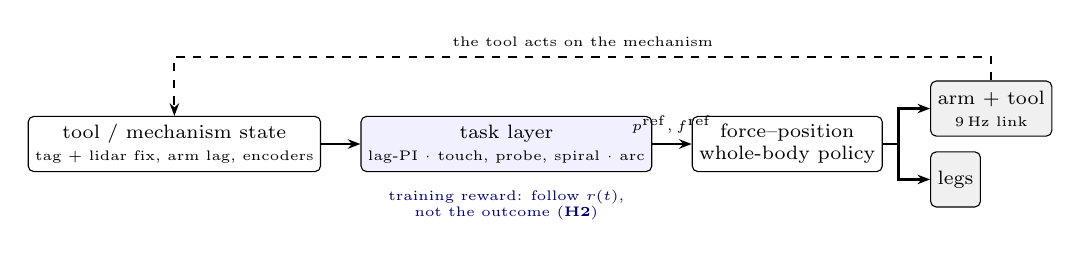
\begin{tikzpicture}[font=\scriptsize, node distance=4mm and 5mm,
  box/.style={draw, rounded corners=2pt, align=center, inner sep=2.5pt, minimum height=7mm},
  hw/.style={box, fill=black!6}, arr/.style={-{Stealth[length=1.6mm]}, thick}]
\node[box] (obs) {tool / mechanism state\\{\tiny tag + lidar fix, arm lag, encoders}};
\node[box, right=of obs, fill=blue!6] (layer) {task layer\\{\tiny lag-PI $\cdot$ touch, probe, spiral $\cdot$ arc}};
\node[box, right=of layer] (pi) {force--position\\whole-body policy};
\node[hw, right=6mm of pi, yshift=4.5mm] (arm) {arm + tool\\{\tiny 9\,Hz link}};
\node[hw, right=6mm of pi, yshift=-4.5mm] (legs) {legs};
\draw[arr] (obs) -- (layer);
\draw[arr] (layer) -- node[above, font=\tiny]{$p^{\mathrm{ref}}, f^{\mathrm{ref}}$} (pi);
\draw[arr] (pi.east) -- ++(2mm,0) |- (arm.west);
\draw[arr] (pi.east) -- ++(2mm,0) |- (legs.west);
\draw[arr, dashed] (arm.north) -- ++(0,3mm) -| node[above, pos=0.25, font=\tiny]{the tool acts on the mechanism} (obs.north);
\node[font=\tiny, below=1mm of layer, align=center, text=blue!50!black] (rw) {training reward: follow $r(t)$,\\not the outcome (\hyp{2})};
\end{tikzpicture}}
\caption{The task layer turns a tool's or mechanism's state into force--position references for a learned whole-body
policy. A position-only twin receives the same references with $f^{\mathrm{ref}}$ replaced by a depth.}
\label{fig:system}
\end{figure}

%------------------------------------------------------------------------------
\section{Task-Layer References}
\label{sec:layer}

The layer maps a tool or mechanism state $s$ to a reference $r(t) = (p^{\mathrm{ref}}, f^{\mathrm{ref}})$ for the policy
(Fig.~\ref{fig:system}).
It runs at the policy rate in training and on hardware, and is written so that its decisions can be logged and
audited.

\textbf{Mechanisms (T1).} With the handle's lag $e$ behind its goal, $f^{\mathrm{ref}} = \mathrm{sat}_{f_{\max}}
\left(K_p e + K_i \!\int\! e\right)$ along the goal direction. $f_{\max}$ is a task-level force budget.

\textbf{Insertion (T2).} The layer approaches along the estimated keyway axis. It senses the lock face by the arm's lag,
not a force sensor (3\,mm), then makes a 3\,mm sideways probe: if the key is held, it is in the keyway. Otherwise it runs
a spiral search with the wrist rolling. It then presses to the floor, jiggles if stuck, and holds. The force-aware twin
is commanded a press force. The position-only twin is commanded a depth.

\textbf{Turning (T3).} An arc reference $\theta^{\mathrm{ref}}(t)$ for the key's angle, with the foot pressing on the
lever while the arm holds the key's shaft in the keyway.

\textbf{Reward: following the reference.} A reward that pays the outcome ($\theta$, latch open) leaves the policy free to
reach it any way it can. We instead pay progress only up to the reference and price running ahead of it:
\begin{equation}
r_{\mathrm{turn}} = w_p \min(\theta, \theta^{\mathrm{ref}}) - w_a \max(0,\, \theta - \theta^{\mathrm{ref}} - \delta),
\end{equation}
paid only while the layer is pressing or holding.

%------------------------------------------------------------------------------
\section{Hypotheses}
\label{sec:hyp}

\hyp{1} \emph{Task-layer references.} With the same policy architecture and budget, a policy trained with the task layer
in the loop succeeds on more tool tasks, within a force budget, than an outcome-trained policy given only the tool goal.
It also beats a position-scripted controller with the same perception and grasp. \emph{Falsified if} the outcome-trained
policy matches the layer-in-the-loop policy on success and on force-budget violations across three seeds.

\hyp{2} \emph{Pay the reference, not the outcome.} Outcome rewards let the policy reach the goal by a route the layer did
not plan and hardware cannot execute. Paying for following the reference removes this at no loss of success.
\emph{Falsified if} outcome-trained policies follow the reference as closely (fraction of contacts that run ahead, peak
tool speed), or if the following reward costs success across seeds.

\hyp{3} \emph{Force awareness with a tool is conditional.} Between matched twins, the force-aware one wins when the body
or actuation departs from training (leg mass, delay, stance) and when force must be regulated along a reference. The
position-only one is as good or better under nominal conditions and under tool or lock geometry shifts, because pressing
by depth is more precise when the geometry is the uncertainty. \emph{Falsified if}, over three seeds from a common parent,
the difference between twins shows no interaction with the type of shift.

\hyp{4} \emph{Tool conditioning.} A force-aware policy given explicit tool descriptors generalizes to held-out tools
better than the same policy trained on the same tools without them. The descriptors are tip offset and axis, length, grip
compliance and mass. \emph{Falsified if} on held-out tools the descriptor-conditioned policy is no better than the
unconditioned one, or no better than a single-tool policy, within seed variation.

%------------------------------------------------------------------------------
\section{Preliminary Results}
\label{sec:results}

All learned results are simulation, one training seed per variant unless stated, with checkpoints selected on the frozen
sets they are scored on. Stage~2 repeats them on held-out sets with three seeds (Sec.~\ref{sec:plan}).

\textbf{Position scripting on hardware (motivation for \hyp{1}).} The scripted sequence uses camera and lidar fixes of a
tagged box, a holster for the key, arm inverse kinematics, and the vendor's walking controller. On the real robot it ran
the whole chain (unlock, pull, close, lock) to completion in 5 of 11 runs, three of the six failures being operator stops.
It once opened, closed and locked the box in a single run. Its failures were at contact. A position-aimed press pushed
the key 66\,mm past seated, shutting the door ahead of it, and in another run 35\,mm past seated without stopping. A
2\,mm offset between grip and shaft turned a 45$^\circ$ command into 33.5--34.3$^\circ$. In simulation, the same stack
seated 0 of 12 keys from its camera fix, because a 3--11\,mm range error along the keyway stalls a position-aimed push.

\textbf{\hyp{1}: the layer makes a force channel usable for tool goals} (Table~\ref{tab:h1}). Commanded only by where a held handle should go,
no existing policy found the force. The 60\,N pull policy drove at most about 30\,N. A policy trained on the outcome alone
stopped at the same 30\,N, because nothing paid for pushing harder before the mechanism moved. The PI law on the handle's
lag, with no retraining, made the pull policy open 337 of 480 held mechanisms (70\,N drawers, 60\,N latches) and fail safe
beyond its capacity. An end-to-end policy given only the goal, once pushing was paid, opened 358. Trained with the layer
in the loop, the policy opened \textbf{504 of 512} held-out mechanisms, including a button the others could not press.
It leaned back into pulls and forward onto pushes. With the same layer and a modelled claw (still on the idealized arm), it opened the combiner box
in 16 of 16 placements against door closers up to 16\,N$\cdot$m. The same claw and script on the position-tracking policy
opened 9 of 16 free doors and none from 8\,N$\cdot$m. On the insertion, the learned whole body with the touch-sensing layer
seated 66--81 keys inside the tilt stop, against 11--25 for a classical 10\,Hz IK arm on the same legs. On the key hold,
the trained policies unlocked and kept 104--108 of 108 (on a 50\,Hz arm and on the D1's interface). Pairing the same
legs with a classical IK arm gave 18, and fixing the arm's joints gave none. A whole-hand pose policy on the door and lever opened 32 of 32 doors and did the lever then the door
31 of 32 times, against 18 and 4 for a position-commanded policy with a wrist servo.

\begin{table}[t]
\centering
\caption{Task-layer references against their alternatives (simulation unless marked). Counts are successes.}
\label{tab:h1}
\footnotesize
\setlength{\tabcolsep}{2.5pt}
\begin{tabular}{@{}p{0.26\columnwidth}p{0.19\columnwidth}p{0.49\columnwidth}@{}}
\toprule
task (set) & layer in the loop & alternatives \\
\midrule
T1 held mechanisms & 504 / 512 & law zero-shot 337 / 480; outcome-trained 358 / 480; pull policy alone stalls at $\approx$30\,N \\
T1 combiner box, claw (16) & 16, closers to 16\,N$\cdot$m & position-tracking policy, same script: 9 free doors, 0 from 8\,N$\cdot$m \\
T2 key insertion (96) & 66--81 & classical 10\,Hz IK arm, same legs: 11--25 \\
T3 key hold (108) & 104--108 & same legs, IK arm: 18; arm fixed: 0 \\
T4 door; lever then door (32) & 32; 31 & position command, wrist servo: 18; 4 \\
\midrule
key chain, \emph{real robot} & not yet run & position script: 5 / 11 complete \\
\bottomrule
\end{tabular}
\end{table}

\textbf{\hyp{2}: outcome rewards bypass the layer.} Every key-hold policy rewarded for the key's angle and the open latch
turned the key in one stroke ahead of the layer's arc: 45$^\circ$ in about 0.1\,s (460--600$^\circ$/s), in nearly every
unlock, then traced the arc in the air. The wrist's lead peaked at 40--46$^\circ$. Paying the turn only up to the
reference and pricing a run ahead of it (Eq.~1) removed the snap in both twins. No key in 911 unlocks ran ahead, the turn
took 1.2--1.5\,s, and the wrist's lead fell to 13--23$^\circ$. The force-aware policy kept its success. A related effect
appears with force budgets: with the outcome reward in training, the policy treated the layer's 40\,N cap as advice
(146 of 180 heavy mechanisms opened past it), while a pure force-follower stayed nearer the cap and lost capacity (56).

\begin{figure}[t]
\centering
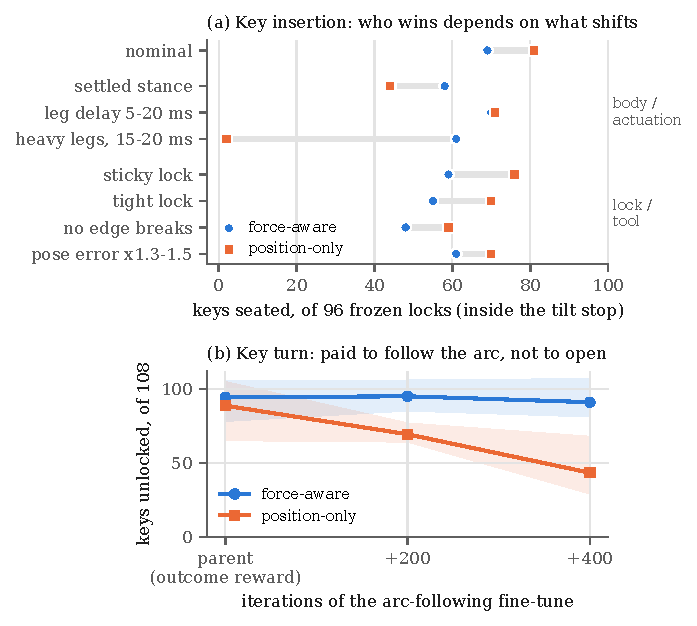
\includegraphics[width=\columnwidth]{figures/fig_matched.pdf}
\caption{Matched twins in simulation. (a) Key insertion, force-aware against position-only (one selected checkpoint
each), scored on held-out shifts of the body and actuation or of the lock and tool. (b) Key turn: success averaged over
three stance and friction conditions (band: their range) while fine-tuning with the reference-following reward (Eq.~1)
from parents trained on the outcome.}
\label{fig:matched}
\end{figure}

\textbf{\hyp{3}: force awareness is conditional.} Fig.~\ref{fig:matched}a shows the insertion twins. Under nominal
conditions position-only seats more (81 against 69). Under lock and tool shifts it stays ahead by 9--17. Under body
and actuation shifts the ranking reverses: from the settled stance 58 against 44, and on heavy legs with a 15--20\,ms
command delay 61 against 2. Fig.~\ref{fig:matched}b shows the key turn under the reference-following reward. The
force-aware twin held 81--107 of 108 through 400 iterations. The position-only twin fell to 29--68: its failures are
stalls, the foot on the lever and the key stopped about 26$^\circ$ against a latch at 30$^\circ$, 13--15$^\circ$ behind
the reference. This pattern also corrects one of our own earlier readings. A force-aware lead on stiffer locks
(79 against 45) disappeared when a position-only fine-tune was trained on the same lock range (104 against 94), so it was
a training-range effect, not a property of the force channel.

\textbf{Force through a tool on hardware.} The deployed whole-body policy (trained through the identified arm interface)
pressed a cloth on a bench through its force input, open loop. On a scale, the measured force rose from 7 to 19\,N as the
command went from 0 to 6\,N, about 2\,N per commanded newton. The foot-contact sensors tracked it to about 1\,N at that
pose. Eight force-commanded wipes ran without a stop, with the estimated force rising with the command (about 2 to 21\,N).
No learned key, lever or door policy has run on the robot yet.

%------------------------------------------------------------------------------
\section{Planned Experiments}
\label{sec:plan}

Every comparison uses three training seeds, matched transition budgets, selection on a validation set, and an untouched
test set. Every hardware trial is counted, aborts included.

\textbf{E1 (\hyp{1}): the layer against its alternatives.} On T1--T3, under the same architecture and budget, we compare
(i) layer in the loop, (ii) the layer applied zero-shot to a policy not trained with it, (iii) an outcome-trained policy
given only the tool goal, and (iv) the position script. Measures: success, force-budget violations, peak contact force.

\textbf{E2 (\hyp{2}): reference against outcome reward.} Both rewards on T2 and T3, from a common parent. Measures:
success, fraction of contacts that run ahead of the reference, peak tool speed, wrist lead, and keys lost after unlocking.

\textbf{E3 (\hyp{3}): a factorial of shifts.} Twins fine-tuned from one common parent, which removes the confound in the
present lineages, where the twins have different parents. They are scored on a grid crossing body shifts (leg armature,
delay, stance) with tool shifts (lock stiffness, tightness, pose error, tool length). We will test the twin $\times$ shift
interaction with a mixed-effects model over seeds and conditions.

\textbf{E4 (\hyp{4}): tool conditioning.} A procedural family of keys (length, shaft offset, bow shape), claws (lip depth,
jaw clearance) and pads (thickness, compliance), with mass and grip compliance varied. We will train three policies on
the same tools and transitions: a force-aware policy without descriptors, the same with descriptors, and single-tool
specialists. All are tested on held-out tools at the extremes and in the gaps of the training range. We also test
whether a descriptor wrong by a known amount degrades the policy gracefully.

\textbf{E5 (hardware).} The force-aware insertion and the position script on the real cam lock, 20 trials across four
box placements, with a load cell behind the lock. Measures: seated, overshoot past seat, peak force, time. Force-aware
against position-only wiping on a force plate, with erased area scored against a fixed pattern. Policies are screened
first on replayed real proprioception from the robot.

%------------------------------------------------------------------------------
\section{Limitations}

The learned results are simulation. The lock, latch and door are analytic plants with drawn stiffnesses, the key is
tied to the hand by a spring, and the insertion contact is softer than PLA on metal. The frozen sets were used for both
selection and scoring, mostly with one seed, and the twins in Fig.~\ref{fig:matched} come from different parents. Some
policies are fragile to leg conditions outside their training, and key-hold training broke in every run at UniFP's
learning rate. No learned tool policy has run on the robot, and the force channel on hardware is open loop. \hyp{4} has
no evidence yet.

%------------------------------------------------------------------------------
\section{Conclusion}

Force--position control gives a legged manipulator a way to push. A tool task still has to say how hard, in which
direction, and when. Our preliminary evidence suggests three things. A thin task layer that turns tool state into
force--position references is what makes a learned force channel useful for tools. The policy must be paid to follow
that layer, not to reach the outcome. Force awareness earns its place under the body and actuation uncertainty a real
legged robot has, more than under tool geometry. The proposed experiments test these claims and whether telling the
policy about its tool lets one controller serve many.

\bibliographystyle{plainnat}
\bibliography{references}

\end{document}
